% Section content template for individual Educative lessons
% This file contains the actual content for a specific section
% Generated from Educative API section content

% Section: Requirements of the Typeahead Suggestion System’s Design
% Section ID: 6369391511339008
% Section Slug: requirements-of-the-typeahead-suggestion-systems-design
% Generated: 2025-12-08T15:11:14.985626

\subsection{Requirements}\label{k7Y2v_ciUumvCx5muSkt3}
\\
In this lesson, we look into the requirements and estimated resources that are necessary for the design of the typeahead suggestion system. Our proposed design should meet the following requirements.

\subsubsection{Functional requirements}\label{j21JdNbSCrgDlISuZn1I8}
\\
The system should suggest top \protect\phantomsection\label{katex_inline_3NM0FAhcZ70ijcHvOc4sW}{{{\(N\)}}} (let's say top ten) frequent and relevant terms to the user based on the text a user types in the search box.

\subsubsection{Non-functional requirements}\label{uEzqyTpZALCY0Y3tiMDm0}

\begin{itemize}
\item
\protect\phantomsection\label{oOVSMHriSX2vvV9YMkcga}
\textbf{Low latency:} The system should show all the suggested queries in real time after a user types. The latency shouldn't exceed 200 ms. A study suggests that the average time between two keystrokes is 160 milliseconds. So, our time budget of suggestions should be greater than 160 ms to give a real-time response. This is because if a user is typing fast, they already know what to search and might not need suggestions. At the same time, our system response should be greater than 160 ms. However, it should not be too high because in that case, a suggestion might be stale and less useful.
\item
\protect\phantomsection\label{mEcE0fNxCKQvLpXvrVkDC}
\textbf{Fault tolerance:} The system should be reliable enough to provide suggestions despite the failure of one or more of its components.
\item
\protect\phantomsection\label{l2QhqwoWt4K1gkL92_FGR}
\textbf{Scalability:} The system should support the ever-increasing number of users over time.
\end{itemize}

\subsection{Resource estimation}\label{59fw27MzCsy3WBsJfFZKe}
\\
As was stated earlier, the typeahead feature is used to enhance the user experience while typing a query. We need to design a system that works on a scale that's similar to Google Search. Google receives more than 3.5 billion searches every day. Designing such an enormous system is a challenging task that requires different resources. Let 's estimate the storage and bandwidth requirements for the proposed system.

\subsubsection{Storage estimation}\label{qGV6V0uwz1NbzqkciJqAb}
\\
Assuming that out of the 3.5 billion queries per day, two billion queries are unique and need to be stored. Let 's also assume that each query consists of 15 characters on average, and each character takes 2 Bytes of storage. According to this formulation, we would require the following: \protect\phantomsection\label{katex_inline_MqdPcTos3CERBOSwcZcZR}{{{\(2 \text{ billion} \times 15 \times 2 = 60 \text{GB}\)}}} to store all the queries made in a day.
\\
Storage required per year: \protect\phantomsection\label{katex_inline_Lf_yXb7QWV3WnMEf5_sAp}{{{\(60\ \text{GB/day} \times 365 = 21.9\ \text{TB/year}\)}}}\\

\begin{figure}[htbp]
 \centering
 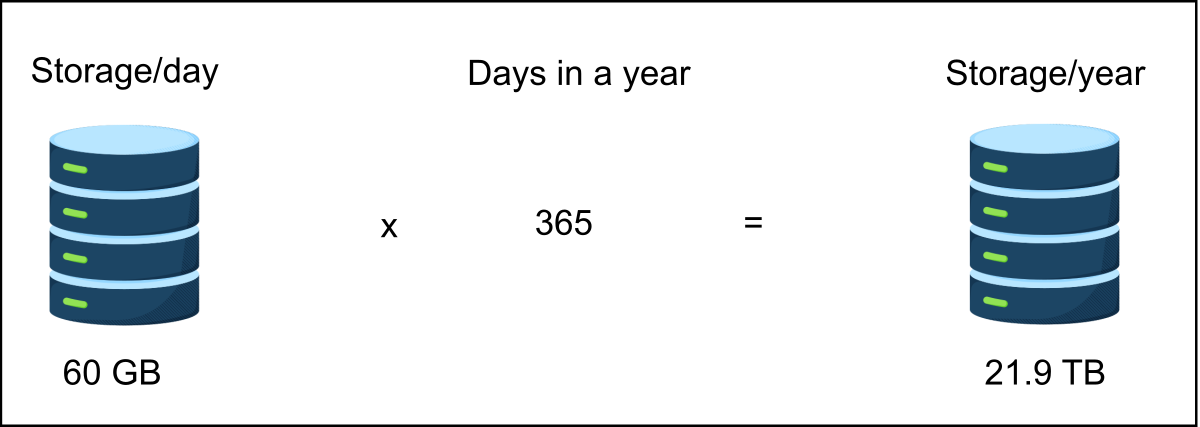
\includegraphics[width=0.5\textwidth]{Images/chapter_37/section_6369391511339008/6366409171271680.png}
 \caption{Storage requirements for the typeahead suggestion system}
\end{figure}

\subsubsection{Bandwidth estimation}\label{VQB9skv8FrrKcrgC2erJI}
\\
3.5 billion queries will reach our system every day. Assume that each query a user types is 15 characters long on average.
\\
Keeping this in mind, the total number of reading requests of characters per day would be as follows:
\\
\protect\phantomsection\label{katex_inline_ZHDC2DNLrnEWjoprJF2a0}{{{\(15 \times 3.5 \text{ billion = 52.5 billion} \)}}} characters per day.
\\
Total read requests per second: \protect\phantomsection\label{katex_inline_21TdxXqpkxA3W065BDx2C}{{{\(52.5\text{B}/86400 \approx 0.607 \text{M}\)}}} characters/sec. 86,400 is the number of seconds per day.
\\
Since each character takes 2 Bytes, the bandwidth our system would need is as follows:
\\
\protect\phantomsection\label{katex_inline_EmoRp2F2ggNr6sAcJUscJ}{{{\(0.607\ \text{million} \times 2 \times 8 = 9.7\ \text{Mb/sec}\)}}}
\\
\protect\phantomsection\label{katex_inline_jcybhXTse6_J1lIc3a8ob}{{{\(9.7\text{ Mb/sec}\)}}} is the incoming bandwidth requirement for queries that have a maximum length of 15 characters. Our system would suggest the top ten queries that are roughly of the same length as the query length after each character a user types. Therefore, the outgoing bandwidth requirement would become the following:

\[
10 \times 9.7\ \text{Mb/sec} = 97\ \text{Mb/sec}
\]

\begin{figure}[htbp]
 \centering
 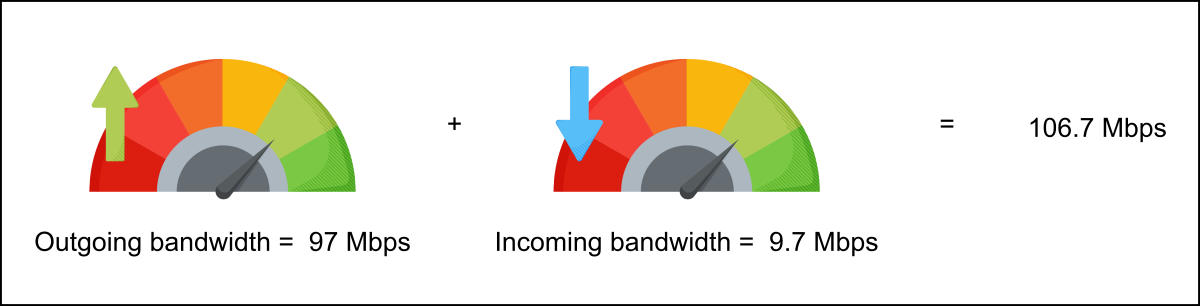
\includegraphics[width=0.5\textwidth]{Images/chapter_37/section_6369391511339008/5686906522566656.png}
 \caption{The total bandwidth required by the typeahead suggestion system}
\end{figure}

\subsubsection{Number of servers estimation}\label{hCasTr81fZVlAFPYDVGWP}
\\
Our system will receive 52.5 billion requests per day. Considering ~\href{https://www.educative.io/courses/grokking-the-system-design-interview/put-back-of-the-envelope-numbers-in-perspective}{our assumption}~of using daily active users as a proxy for the number of requests per second for peak load, we get 52.5 billion requests per second (considering each character as a request).
\\
Recall that a typical server can serve 64,000 requests per second (RPS). So, the required servers can be estimated using the following formula:

\[
\text{Number of servers} = \frac{\text{Number of requests/second}}{\text{RPS of server}}
\]

\[
\text{Number of servers} = \frac{52.5\ \text{billion}}{64,000} = 820312.5 \approx 821 \text{ K servers}
\]

\begin{quote}
The initial estimate of 52.5 billion requests per second seems unrealistic. However, on average, a person types at a rate of around three to four characters per second.
\end{quote}
\\
Therefore, assuming 3.5 billion users and a peak load scenario where each user types roughly three characters per second, we arrive at a more feasible estimate of (\protect\phantomsection\label{katex_inline_Q-47gLjp45ZZOLeL1jyau}{{{\(3.5\times 3\)}}}) billion requests per second. This revised figure provides a more realistic estimation as follows:

\[
\text{Number of Servers} = \frac{3.5\ \text{billion} \times 3}{64,000} = 164062.5 \approx 164\ \text{K servers}
\]

\begin{figure}[htbp]
 \centering
 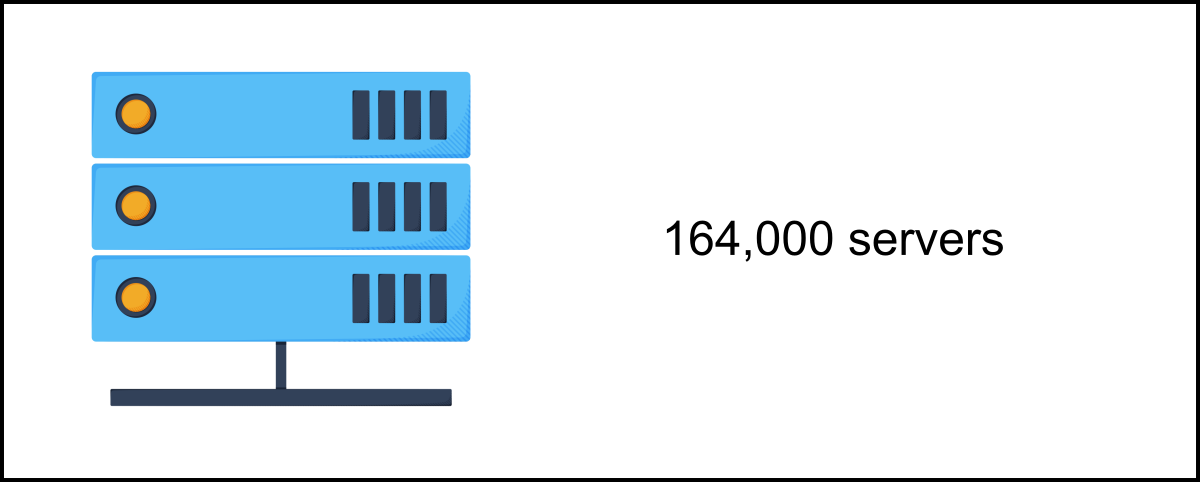
\includegraphics[width=0.15\textwidth]{Images/chapter_37/section_6369391511339008/5601527991762944.png}
 \caption{The number of servers required for the typeahead suggestion system}
\end{figure}

In the table below, adjust the values to see how the resource estimations change.

\subsection{Building blocks we will use}\label{1RAi3BkLVRt85wowy8DOD}
\\
The design of the typeahead suggestion system consists of the following building blocks that have been discussed in the initial chapters of the course:

\begin{figure}[htbp]
 \centering
 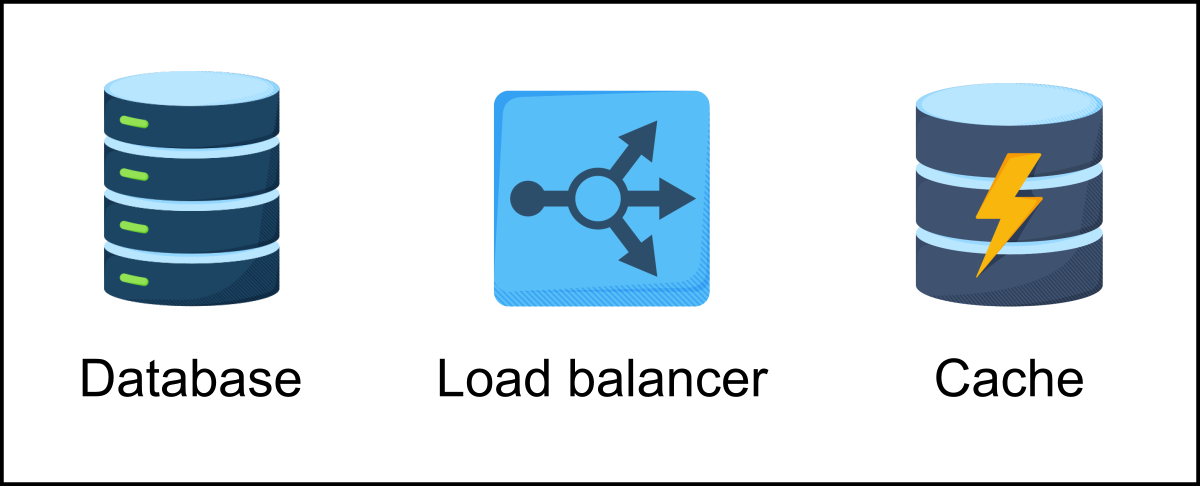
\includegraphics[width=0.25\textwidth]{Images/chapter_37/section_6369391511339008/6448309348990976.png}
 \caption{Building blocks required in the design of the typeahead suggestion system}
\end{figure}

\begin{itemize}
\item
\protect\phantomsection\label{ZiEmogSgTKwNPNLPTwuGT}
\href{https://www.educative.io/courses/grokking-the-system-design-interview/introduction-to-databases}{\textbf{Databases}} are required to keep the data related to the queries' prefixes.
\item
\protect\phantomsection\label{UPKN1bMSVxPNqvRZopp33}
\href{https://www.educative.io/courses/grokking-the-system-design-interview/introduction-to-load-balancers}{\textbf{Load balancers}} are required to disseminate incoming queries among a number of active servers.
\item
\protect\phantomsection\label{Kz6n-yHEKuNk2TsDvW5Jv}
\href{https://www.educative.io/courses/grokking-the-system-design-interview/system-design-the-distributed-cache}{\textbf{Caches}} are used to keep the top N suggestions for fast retrieval.
\end{itemize}
\\
In the next lesson, we'll focus on the high-level design and APIs of the typeahead suggestion system.

% End of section content